\documentclass[11pt]{article}

\usepackage[margin=1.1in]{geometry}
\usepackage{amsmath,amssymb,amsthm}
\usepackage{stmaryrd}
\usepackage{mathtools}
\usepackage{tikz}
\usetikzlibrary{arrows.meta,positioning,fit,backgrounds,patterns,calc,decorations.pathmorphing}
\usepackage{listings}
\usepackage{xcolor}
\usepackage{booktabs}
\usepackage{array}
\usepackage[colorlinks=true,linkcolor=black,citecolor=black,urlcolor=blue]{hyperref}
\usepackage[expansion=false]{microtype}

\theoremstyle{plain}
\newtheorem{theorem}{Theorem}
\newtheorem{proposition}[theorem]{Proposition}
\newtheorem{lemma}[theorem]{Lemma}
\newtheorem{corollary}[theorem]{Corollary}
\newtheorem{conjecture}[theorem]{Conjecture}
\theoremstyle{definition}
\newtheorem{definition}[theorem]{Definition}
\newtheorem{remark}[theorem]{Remark}
\newtheorem{observation}[theorem]{Observation}
\newtheorem{question}{Question}

% --- typography: the rho calculus is NEVER written with the Greek letter ---
\newcommand{\rhoc}{\textsf{rho}}
\newcommand{\Chn}{\mathrm{Chn}}
\newcommand{\bt}{b_{\mathrm{t}}}

\lstdefinestyle{rho}{
  basicstyle=\ttfamily\small,
  keywordstyle=\bfseries,
  morekeywords={for,new,in,def,where,contract,match,if,else,Nil},
  columns=fullflexible,
  showstringspaces=false,
  breaklines=true,
  frame=none,
  xleftmargin=1.5em,
  comment=[l]{//},
  commentstyle=\itshape\color{black!55},
}
\lstset{style=rho}

\title{\bfseries Feeding the Colony\\[.35em]
\large Transport architectures for tubular agents, and where the vascular tree comes from}
\author{L.\ G.\ Meredith\\ \small F1R3FLY.io}
\date{September 11, 2026}

\begin{document}
\maketitle

\begin{abstract}
The tube note \cite{tubenote} argues that a phagotrophic agent is topologically a tube, and its
companion chapter observes that a digestive organ is a community of learners tenanted in a boundary
namespace. Put the two together with the individuation threshold of the engine note and a second
problem appears immediately. A tubular agent is colonial in two distinct senses; extraction happens
at a boundary, and consumption happens throughout a volume; so the yield has to be moved. This note
argues that the transport problem so posed is not a new problem but the isoperimetric inequality
already used to individuate an agent, read a second time as supply against demand; that the vascular
bed is the lumen construction applied recursively, whose function is to manufacture boundary in the
interior; that the two-ends proposition recurses, so that a single-named circulation must alternate;
and that the tube criterion itself is scale-free, giving the closed circulatory system as the same
statement one level in. It then examines the instinct that the situation calls for optimal transport.
Monge--Kantorovich transport is argued to be the wrong object, since it yields a plan rather than an
architecture and requires mass conservation that dissipation denies. Branched transport is the right
object, and the framework's contribution is that it does not have to postulate the concavity that
branched transport assumes: reflection supplies it, because one rendezvous moves a quoted term of any
size, while contention on a shared name supplies the countervailing convex term. The exponent is
therefore fixed by the pricing schedule rather than chosen. The sharpest consequence is a conflict.
Strictly concave transport optima are acyclic, while the engine note's Foster theorem prices the
detection strength of a price code by the first Betti number, which is zero on a forest. A
transport-optimal network cannot be regulated. Vasculature must therefore sit off the transport
optimum by exactly its regulatory capacity. A ladder of seven minimal transport architectures is
given, together with a currency argument whose conclusion is that the circulating carrier is the
virtual token given a medium. As with its sibling, this is a research note in the strict sense: an
argument, a list of statements to attempt, the empirical checks each would face, and an account of
where it is weakest.
\end{abstract}

\section{The proposition}
\label{sec:obs}

\emph{Dictated 11 September 2026.}

Tubular agents have been described as colonial, in the sense that such an agent is a colony of
agents. When such an agent extracts resources, whether by digestion or by respiration, it must
disseminate those resources to the colony. That requirement appears to call for optimal transport,
and it suggests that the architecture of vascular systems arises directly from the framework rather
than being an additional biological fact to be accommodated.

The tube note's sixth open question asks exactly this and leaves it open: where does circulation
enter, and does the vascular tree follow from the tube together with an allometric constraint? The
argument below answers yes to the second half and disputes the premise of the first. What does the
work is not allometry but the individuation threshold, and allometry is a consequence rather than a
co-premise.

\section{What the framework already supplies}
\label{sec:imports}

As with the tube note, the claim here is that the pieces are on the table and the architecture
follows.

\paragraph{Individuation as a ball.} The engine note defines an individual as a region $B$ of the
engine graph that may close over its namespace, and gives the criterion isoperimetrically:
$h(B) = |\partial B| / |B| \geq \kappa r$ with $\kappa = \varepsilon\theta/\rho$, the individual being
the largest ball satisfying it. On a graph of polynomial growth this recovers a finite critical
radius $r^{*}$; under expansion it becomes linear and the merged population grows exponentially in
the radius.

\paragraph{Dissipation along a pathway.} Value is non-increasing along engine operations, and along a
path of length $d$ in the cost metric the delivered value is $\nu e^{-\theta d}$. Against a
round-trip toll linear in $d$, a conversion at distance $d$ is profitable exactly on an interval
$[0, d^{*})$, with $d^{*}$ the unique root of $Y e^{-\theta d} = cd$. There is a horizon on
conversion set by metering rather than by any speed limit.

\paragraph{Cycles price the code.} The engine note's Foster theorem gives the total strength of a
price code as $\bt$, the first Betti number of the relevant graph, and its corollary records that a
thin pathway is uncorrectable for two independent reasons: nothing checks its rates, and nobody owns
its medium.

\paragraph{Flavor incommensurability.} Tokens held in a foreign flavor cannot pass without an enzyme
linking the flavors. This is what makes gut depth track flavor distance in the tube note's
Proposition~H, and it is what will make a single circulating currency cheap in
Section~\ref{sec:currency}.

\paragraph{The lumen is outside.} The tube note's central observation: the interior of the tube is
boundary namespace, owned but open. A tube is the construction that surrounds a region of the outside
with the inside.

\paragraph{The boundary namespace can be let.} The companion chapter's observation: a population of
learners occupying $\Chn_{\partial}(B)$ is neither part of $B$'s internal computation nor foreign to
it, so a digestive organ is a community tenanted in a boundary namespace.

\paragraph{Two ends, not one.} The tube note's Proposition~D: intake and expulsion must sit on
distinct names, since on a shared channel an offer of refuse and a receipt for intake rendezvous.

\paragraph{The tube criterion.} The tube note's Proposition~I: a tube is forced when the agent is
phagotrophic, the occupancy ratio $\Lambda = \tau_{\mathrm{proc}}/\tau_{\mathrm{enc}}$ is at least of
order unity, and the separability $\mu$ is near zero.

\section{Two colonies, three transport problems}
\label{sec:two}

The colonial claim has to be made twice, because the two colonies are different populations and only
one of them has a transport problem.

The colony of the companion chapter's letting observation is tenanted in $\Chn_{\partial}(B)$. It
sits at the extraction site. Whatever it converts, it converts where the material already is, and
nothing has to be moved to reach it.

The colony that the dictated proposition is about is the interior, and its colonial status comes from
a different result. By the individuation criterion an individual is a \emph{ball} in the engine
graph, and a ball is a population; by the tower, the outside of one level is the inside of the next,
so the members of that population are themselves individuals with their own stacks and their own burn
rates. The interior is colonial by the individuation theorem rather than by the lumen observation.
The distinction matters because it is the individuation theorem that also supplies the inequality the
transport problem turns out to be.

Three problems follow, of which the proposition names one.

\begin{enumerate}
\item \textbf{Supply the tenants.} Trivial: they are at the source.
\item \textbf{Supply the interior.} Each member of the interior population has a burn rate $b_i$ and
a residual life $\sigma_i / b_i$. Demand is distributed over $|B|$; supply arrives on
$\Chn_{\partial}$.
\item \textbf{Clear the interior.} The interior population produces its own residue, which is not the
gut's residue and does not leave by the gut's expulsion name.
\end{enumerate}

Problem 3 is the one most easily overlooked, and Section~\ref{sec:ladder} locates it: it is what the
seventh architecture is for.

\begin{figure}[t]
\centering
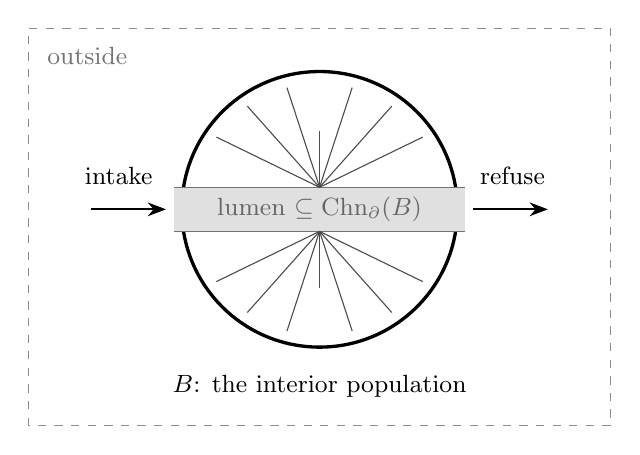
\begin{tikzpicture}[scale=1.0]
  % outside
  \draw[dashed,black!45] (-3.7,-2.75) rectangle (3.7,2.3);
  \node[black!55,font=\small] at (-2.95,1.95) {outside};
  % the individual
  \draw[very thick] (0,0) circle (1.75);
  \node[font=\small] at (0,-2.25) {$B$: the interior population};
  % the lumen: a channel through
  \fill[black!12] (-1.85,0.28) -- (1.85,0.28) -- (1.85,-0.28) -- (-1.85,-0.28) -- cycle;
  \draw[black!55] (-1.85,0.28) -- (1.85,0.28);
  \draw[black!55] (-1.85,-0.28) -- (1.85,-0.28);
  \node[font=\small,black!60] at (0,0) {lumen $\subseteq \Chn_{\partial}(B)$};
  % arrows in and out
  \draw[-{Stealth},thick] (-2.9,0) -- (-1.95,0);
  \draw[-{Stealth},thick] (1.95,0) -- (2.9,0);
  \node[font=\small] at (-2.55,0.42) {intake};
  \node[font=\small] at (2.45,0.42) {refuse};
  % the transport net: ramification off the lumen into the bulk
  \foreach \a in {35,55,75,105,125,145} {
    \draw[black!70] (0,0.28) -- (\a:1.6);
  }
  \foreach \a in {215,235,255,285,305,325} {
    \draw[black!70] (0,-0.28) -- (\a:1.6);
  }
  \draw[black!70] (0,0.28) -- (0,1.0);
  \draw[black!70] (0,-0.28) -- (0,-1.0);
\end{tikzpicture}
\caption{Supply is supported on the boundary namespace; demand is supported on the bulk. The
transport network carries $\Chn_{\partial}$ into the interior so that every member of the interior
population lies within the profitable radius $d^{*}$ of a boundary rendezvous.}
\label{fig:three}
\end{figure}

\section{The transport problem, and the inequality it already is}
\label{sec:problem}

\begin{proposition}[Supply is boundary-supported, demand is bulk-supported]
\label{prop:J}
Extraction rendezvous occur on $\Chn_{\partial}(B)$, so the supply measure is supported on $\partial
B$. Every member of the interior population has a nonzero burn rate, so the demand measure is
supported on $B$ with weights $b_i$. Sustainability of the individual is a relation between a
boundary term and a bulk term whose ratio is $h(B)$.
\end{proposition}

The content of Proposition~\ref{prop:J} is not that a transport problem exists but that the framework
has already written down the inequality governing it. The individuation criterion balances repair
delivered through a cross-section against error accumulated in a volume. Replace repair by yield and
error by burn and the inequality is unchanged in form. \emph{The vascular problem is the
isoperimetric criterion read a second time.} Nothing new is assumed, which is the same claim the tube
note makes for the tube, and it is why this note treats allometry as downstream: exponents in body
size follow from a criterion about boundaries, not the other way around.

\begin{proposition}[Transport is the lumen construction, recursed]
\label{prop:K}
A transport network is a sub-namespace of $\Chn_{\partial}$ embedded in a region already enclosed. Its
function is to raise the effective $h(B)$ without lowering $r$: it manufactures boundary in the
interior.
\end{proposition}

If Proposition~\ref{prop:K} goes through then the gut and the capillary bed are one construction at
two levels of the tower, exactly as the gut and the mycorrhizal network were one access profile on
two sides of an ownership line. The vascular system is not a second kind of thing that large bodies
happen to acquire. It is what the lumen observation says, applied again.

\begin{corollary}[Bed density is set by $\theta$]
\label{cor:krogh}
Every member of the interior population must lie within $d^{*}$ of a supply point, since beyond
$d^{*}$ delivery does not repay its own toll. Hence the spacing of terminal supply points is
$2 d^{*}$ in the cost metric.
\end{corollary}

This is the Krogh cylinder \cite{krogh1919} obtained as a consequence rather than assumed as a
physiological datum, and the prediction it carries is specific and awkward enough to be worth testing:
terminal bed density should track $\theta$, the per-hop conversion loss along the delivery chain,
rather than tracking gross demand. Two tissues with equal oxygen consumption but different conversion
depth should differ in capillary density.

The pure case is instructive. The insect tracheal system delivers by extending the outside to every
cell: no carrier, no currency, no return path. Nothing is converted en route, so $\theta$ is whatever
diffusion costs and $d^{*}$ is short. The known ceiling on insect body size is then the framework's
ceiling, reached at exactly the point where the architecture has no remaining way to manufacture
interior boundary.

\section{Two ends again}
\label{sec:twoends}

\begin{proposition}[The two-ends argument recurses]
\label{prop:L}
Delivery and collection cannot share a name, by the rendezvous argument of the tube note's
Proposition~D applied one level in: an offer of spent carrier and a receipt for fresh carrier will
rendezvous. A circulation on a single name is therefore not impossible but rate-limited by a mutual
exclusion, and must time-share.
\end{proposition}

Time-sharing on a single vessel means the flow must reverse, and the empirical situation is
unusually favourable. In tunicates the peristaltic heart reverses the direction of pumping
periodically, typically every one to three minutes, and no physiological advantage for the reversal
is commonly accepted \cite{konrad2016,kriebel1968}; the phenomenon has been known since the
nineteenth century and the standing explanation, that the pacemakers simply exhaust themselves, was
already being contested fifty years ago \cite{heron1975}. Periodic heart-beat reversal is likewise
documented across four orders of holometabolous insects \cite{gerould1933}, whose dorsal vessel is
again a single tube. Vertebrates, whose arterial and venous namespaces are distinct, do not reverse.

Proposition~\ref{prop:L} predicts a duty cycle in transport exactly as Proposition~D predicts one in
feeding, and the cnidarian check and the tunicate check are the same check at two levels. What makes
the second more interesting than the first is that it attaches to an observation the physiology
literature has left unexplained.

\section{The criterion is scale-free}
\label{sec:scalefree}

\begin{proposition}[Closure is the tube criterion, one level in]
\label{prop:M}
Proposition~I transfers with its two parameters reinterpreted. $\Lambda$ becomes trunk occupancy, the
residence time of a delivered load over the interval at which a further load could profitably be
dispatched. $\mu$ becomes the degree to which spent carrier can leave past fresh carrier at the same
aperture. A \emph{closed} circuit is forced when the carrier is structured rather than a bare token,
$\Lambda \gtrsim 1$, and $\mu \approx 0$; failure of any one is sufficient for an open circulation.
\end{proposition}

Open circulation is the bag of transport. Hemolymph is miscible with the interstitial space and
returns through sinuses, which is $\mu \approx 1$, and the criterion is not met. The condition that
does the real work in Proposition~\ref{prop:M} is the first one.

\begin{observation}[A carrier that is a term must come home]
\label{obs:carrier}
A carrier that is a token can be spent and abandoned. A carrier that is a \emph{quoted converting
term} --- a pigment, an enzyme in transit --- cannot: it has to return to be recharged, and a return
path on a name distinct from the delivery name is a cycle.
\end{observation}

Observation~\ref{obs:carrier} gives a cut that is not body size. Closed circulation should correlate
with a recovered and recycled carrier rather than with bulk, which puts cephalopods, annelids and
vertebrates on one side and the rest of the molluscs and arthropods on the other, and predicts that
the exceptions to a size correlation will be exactly the animals whose carrier is disposable. It is
worth recording that the open/closed status of the tunicates is itself contested on anatomical
grounds \cite{konrad2016}, which the framework would regard as the expected situation for an animal
sitting at the criterion's boundary.

\section{Which optimal transport}
\label{sec:ot}

The dictated proposition says that the situation cries out for optimal transport. It does, but not
for the theory that phrase usually names, and saying why sharpens the claim considerably.

\subsection{Why Monge--Kantorovich is the wrong object}

Two reasons. First, the Monge--Kantorovich problem returns a transport \emph{plan}, and its optima are
realisable by independent straight paths; nothing in it prefers a shared trunk, so it predicts no
architecture at all. Second, it is a problem about measures of equal mass, whereas transport here is
lossy by construction: what arrives is $\nu e^{-\theta d}$ and the supply and demand masses do not
agree. The decay can be absorbed into an additive cost in the $\theta$-weighted path length, but the
profitable radius cannot: beyond $d^{*}$ delivery is not expensive, it is worthless, and a formalism
without a horizon will not say so.

\subsection{Branched transport, and the concavity the framework does not have to assume}

The right object is the branched or ramified transport problem: Gilbert's minimum-cost communication
networks \cite{gilbert1967}, the Eulerian formulation of Xia \cite{xia2003}, the irrigation patterns
of Maddalena, Morel and Solimini \cite{mms2003}, and the monograph of Bernot, Caselles and Morel
\cite{bcm2009}. There the cost of moving mass $m$ per unit length is $\tau(m)$ with $\tau$ concave,
typically $m^{\alpha}$ for $\alpha \in [0,1)$; concavity may be weakened to subadditivity, which is
exactly the statement that moving mass in bulk is cheaper than moving it separately. Subadditivity is
what produces branching, and the resulting minimisers are trees.

Every treatment of branched transport known to the author of this note takes $\tau$, or the exponent
$\alpha$, as given. The framework does not have to.

\begin{proposition}[Reflection makes hop cost payload-independent]
\label{prop:N}
A rendezvous in \rhoc{} moves a quoted term. Since $@P$ carries a stack of arbitrary size in a single
rewrite, the metered cost of a hop counts rendezvous rather than mass, so $\tau$ is subadditive, and
in the limiting case constant in $m$. Contention supplies the countervailing term: a trunk is a
shared name, a shared name serialises, and a trunk carrying flux $m$ has occupancy
$\Lambda_{\mathrm{trunk}} = m\,\tau_{\mathrm{rdv}} / \tau_{\mathrm{enc}}$, whose Amdahl-shaped penalty
is convex in $m$. The exponent $\alpha$ is therefore determined by the pricing schedule on the send
and receive rules together with the contention model, and is not a free parameter.
\end{proposition}

Two remarks. First, without the convex term the theory collapses: payload-independent hop cost alone
gives $\alpha = 0$, which is the Steiner limit, maximal branching and trunks of zero width. The
contention term is what keeps the trunk finite, and it is the same $\Lambda$ that the tube criterion
already uses. \emph{The two parameters of Proposition~I reappear as the exponent of a transport
problem.} Second, this is the precise sense in which vascular architecture arises directly from the
framework: not that branching is permitted, but that the quantity everything else hangs on is fixed
rather than fitted. Murray's flux--radius law \cite{murray1926}, the junction-angle balances, and the
allometric exponents of West, Brown and Enquist \cite{wbe1997} are all downstream of $\alpha$ by
standard arguments.

\begin{remark}[The load-bearing check]
\label{rem:check}
Proposition~\ref{prop:N} rests entirely on sends being metered independently of payload size. If the
cost-accounting schedule on the \texttt{cost-accounting-transpiler} branch prices a send by term
size then $\alpha \to 1$, subadditivity fails, and branching leaves the theory. This is checkable in the
repository, and should be checked before anything in this section is relied upon.
\end{remark}

\section{Transport optimality and regulability are in conflict}
\label{sec:conflict}

\begin{proposition}[A transport-optimal network carries no price code]
\label{prop:O}
For strictly concave $\tau$ the optimal flow contains no cycles and is representable as a forest
\cite[Prop.~7.8]{bcm2009}. By the engine note's Foster theorem the total strength of a price code is
$\bt$, the first Betti number, which is zero on a forest, and by its thin-pathway corollary an
acyclic pathway is uncorrectable twice over. Hence a network that attains the branched-transport
optimum cannot be regulated or repaired.
\end{proposition}

The conclusion to draw is not that the optimum is wrong but that vasculature necessarily sits off it,
and that the framework says what the offset buys. The cycles in excess of a spanning tree
\emph{are} the regulatory capacity, measured in the same currency as everything else in the
framework. That yields a scaling claim which is falsifiable and not obviously true: anastomotic
density, meaning $\bt$ per unit volume, should track regulatory and repair demand rather than
transport demand.

Two independent results already point the same way. Katifori, Sz\"oll\H{o}si and Magnasco
\cite{katifori2010} observe that efficiency-optimal transport networks are loopless while dicotyledon
leaf venation carries a high density of functional loops, and show that optimising under random
damage, or under sparse fluctuating load, produces loops in the optimum; Corson \cite{corson2010}
reaches the same conclusion via redundancy. The framework's version is more specific in that it names
the quantity the loops buy and prices it against everything else the agent could have bought instead.

\begin{remark}[Three claims on $\bt$]
\label{rem:three}
Foster wants $\bt > 0$ so that the code can be detected. The no-arbitrage condition around a cycle,
which the book identifies with the Wegscheider condition and hence with a chemical potential, wants
$\bt > 0$ so that a consistent price exists at all. Branched transport wants $\bt = 0$. The
circulatory system is where the three meet, and its topology should be readable as the resolution.
\end{remark}

\section{Minimal transport architectures}
\label{sec:ladder}

The rungs below are ordered by what each adds to the namespace, not by phylogeny. Each is minimal in
the sense that removing its distinguishing feature returns the rung beneath it.

\begin{table}[t]
\centering
\footnotesize
\begin{tabular}{@{}>{\raggedright\arraybackslash}p{0.055\textwidth}>{\raggedright\arraybackslash}p{0.30\textwidth}>{\raggedright\arraybackslash}p{0.26\textwidth}>{\raggedright\arraybackslash}p{0.28\textwidth}@{}}
\toprule
& \textbf{What is added} & \textbf{Ceiling} & \textbf{Instance} \\
\midrule
A0 & nothing & $r < d^{*}$ & acoels, flatworms \\
A1 & $\Chn_{\partial}$ ramified inward & good must be in the intake medium & gastrovascular canals, tracheae \\[.2em]
A2 & a carrier, one name & must alternate & tunicate heart, insect dorsal vessel \\
A3 & a second name, open return & no targeting & arthropod, molluscan circulation \\
A4 & channelled return, $\bt \geq 1$ & minimal regulation & closed circulations \\
A5 & anastomoses, ramified hierarchy & cost of being off the optimum & vertebrate vasculature \\
A6 & a second collection network & --- & lymphatics \\
\bottomrule
\end{tabular}
\caption{Seven minimal transport architectures, with what each rung adds and where it stops.}
\label{tab:ladder}
\end{table}

\paragraph{A0: no transport.} Every member of the interior population lies within $d^{*}$ of the
boundary by geometry. Cost zero; ceiling $r < d^{*}$. This rung is already in the tube note's test
set, under the heading \emph{area instead of length}: flatworms and xenacoelomorphs solve the problem
by not having one. The ladder begins where the test set ends.

\paragraph{A1: extend the lumen.} Ramify $\Chn_{\partial}$ into the interior. No carrier, no currency,
no return. This is Proposition~\ref{prop:K} in its cheapest form, and it buys $r \gg d^{*}$ outright.
The ceiling is that the delivered good must already be present in the intake medium, and the residue
shares the space, so $\mu$ returns as a constraint on the same namespace. The framework separates the
two biological instances sharply: tracheae deliver a token requiring no conversion and are therefore
unconstrained in $\Lambda$, while gastrovascular canals deliver structured prey requiring conversion
in the same space that conveys it, and must therefore run at low $\Lambda$. Cnidarians feed in bouts;
insects breathe continuously. The prediction and the observation agree.

\paragraph{A2: a carrier on a single name.} A distinct medium, on the relay rung of the engine note's
medium ladder rather than the converting rung, pumped along one name. By Proposition~\ref{prop:L} it
must alternate. Section~\ref{sec:twoends} is the evidence.

\paragraph{A3: two names, open return.} Delivery on its own name, return by diffusion into a sinus.
Reversal is no longer required. What is still absent is targeting: the return medium is shared, so
delivery cannot be addressed to a tenant.

\paragraph{A4: a closed circuit.} Delivery and return both channelled, so $\bt \geq 1$ from the
topology alone, and Observation~\ref{obs:carrier} says what forces it. This is the first rung at
which a price code has nonzero strength, and therefore the first rung at which the circulation can be
regulated rather than merely run.

\paragraph{A5: closed, ramified, anastomosed.} $\bt$ raised above its topological minimum and paid for
in transport efficiency, per Proposition~\ref{prop:O}; the branching hierarchy with exponent set by
Proposition~\ref{prop:N}.

\paragraph{A6: a second collection network.} Problem 3 of Section~\ref{sec:two}. The fraction of
carrier that leaves the circuit, together with the interior population's own residue, needs a return
that is not the delivery name --- which is the two-ends proposition once more, now at the level of
the whole transport system rather than of a single vessel.

\section{The currency layer}
\label{sec:currency}

The ladder is about topology. The following argument is orthogonal to it and is, on this note's
reading, the most consequential thing in the analysis.

\begin{proposition}[One currency beats $k$ networks]
\label{prop:P}
Let the interior population hold $k$ distinct flavors. Since tokens in a foreign flavor cannot pass
without an enzyme linking the flavors, there are two designs: $k$ dedicated delivery networks, whose
cost scales as $k$ times the length required to reach every member; or one network carrying a single
flavor, with conversion performed locally at each demand point. The converters in the second design
are already present, since every member of the interior population is itself a converting agent.
Hence the single-carrier design wins above a small threshold in $k$, and the flavor that circulates
is the one minimising summed conversion distance to consumers.
\end{proposition}

A good that is held by everyone, converted by everyone, and minimises the summed cost of conversion
into every other good is a num\'{e}raire. So the framework's answer to why a body transports glucose
and oxygen rather than plumbing each metabolite separately is the same as its answer to why there is
money, and the book has already given that answer: the no-arbitrage condition around a cycle in a
reaction network is the Wegscheider condition, and the potential it is equivalent to is a chemical
potential.

\begin{observation}[The circulating carrier is the virtual token given a medium]
\label{obs:numeraire}
The virtual token of the engine note is an accounting device with no bearer. A closed circulation
supplies the bearer. What circulates is not merely a resource but the unit in which the interior
population's internal prices are quoted.
\end{observation}

Observation~\ref{obs:numeraire} puts a cycle back at the centre, since no-arbitrage is a condition on
cycles, and thereby rejoins Remark~\ref{rem:three} from the other side. The currency argument and the
Foster argument want the same $\bt > 0$ for different reasons.

\section{What a tree buys, and what it does not}
\label{sec:tree}

\begin{proposition}[Diameter, not expansion]
\label{prop:Q}
A ramified tree has diameter logarithmic in the number of terminals, which is what controls
$e^{-\theta d}$ and hence reach against dissipation. It does \emph{not} have isoperimetry bounded
below: on a balanced tree a single edge cut separates a constant fraction of the vertices. So the
expansion theorem, which requires $h \geq h_0 > 0$, is unavailable on an arborescent network.
\end{proposition}

Proposition~\ref{prop:Q} is an open problem rather than a result, and it is the largest one this note
generates. If the transport graph were the individuation graph, then an arborescent vasculature would
fail the individuation criterion and the individual would dissolve, which is false. Two repairs are
available and they are not the same repair. Either the two graphs differ, with individuation running
on a denser signalling and repair graph while transport runs on the tree; or the transport graph must
be mesh-like where it matters, which is to say at the periphery. That capillary beds are meshes rather
than the tips of a tree is evidence for the second, and the anastomoses of Proposition~\ref{prop:O}
are evidence for it too. But the question of which graph the individuation criterion is stated over
has been left implicit throughout the engine note, and this note has now made it load-bearing.

\section{What to write down formally}
\label{sec:formal}

\begin{enumerate}
\item The supply and demand measures of Proposition~\ref{prop:J} as term-level quantities, and the
re-reading of the individuation inequality as a sustainability condition, with an explicit statement
of what changes and what does not.
\item $d^{*}$ as a bound on terminal spacing, with the constant, so that
Corollary~\ref{cor:krogh} becomes a number that can be confronted with capillary densities rather
than a shape.
\item $\Lambda_{\mathrm{trunk}}$ as a metered quantity, and the derivation of $\alpha$ from the
pricing schedule. This is the central technical item and the one on which
Remark~\ref{rem:check} sits.
\item The junction condition. With $\alpha$ in hand, the conserved quantity at a bifurcation should be
$\sum_i m_i^{\alpha}$, and the framework should therefore predict a Murray-type exponent rather than
import one.
\item Proposition~\ref{prop:O} as a Pareto statement: the frontier between delivered value and
$\bt$, with the claim that observed vasculature sits on it and not at either extreme.
\item Proposition~\ref{prop:P} with the threshold in $k$ computed, since a threshold of two would be
uninteresting and a threshold of twenty would be a result.
\item The resolution of Proposition~\ref{prop:Q}: which graph the individuation criterion ranges over.
\end{enumerate}

\section{Open questions}
\label{sec:open}

\begin{question}
Does the pump follow, or is it an addition? Everything above concerns topology and pricing, and
nothing so far forces advection over diffusion except the $d^{*}$ horizon. A pump is a metered
process that shortens the effective path, so it should appear as a purchase of $\theta^{-1}$, but the
note has not derived the point at which that purchase pays.
\end{question}

\begin{question}
Is there a framework-native account of \emph{targeting}? A shared carrier delivers to whoever
rendezvous, which is the perception-must-not-act problem in a third guise. Hormonal signalling on the
carrier is exactly a broadcast on a public channel, and should therefore carry a predictable exposure
to spoofing --- which would connect this note to the deception argument of the gap note rather than to
the tube note.
\end{question}

\begin{question}
Does the second critical point of the tube note's last question --- the ruminant's chambering, and
its deliberate return path --- have a transport reading? Buffering and circulation are both answers to
a throughput mismatch, and the return path in the rumen looks like a cycle bought for the same reason
Proposition~\ref{prop:O} says anastomoses are bought.
\end{question}

\begin{question}
What does the framework say about a transport network that is \emph{grown} rather than designed?
Adaptive-network models produce hierarchical vasculature from local flow-dependent rules. The
framework's own version of that question is whether the growth rule can be a revision move on the
relaxation lattice, in which case the vascular tree is a hypothesis the colony holds about where its
own demand will be.
\end{question}

\begin{question}
Does the osmotroph escape this note entirely? An osmotroph everts the lumen, so it has no interior
population to supply in this sense. If Proposition~\ref{prop:K} is right, the fungal mycelium should
be the transport architecture of an agent that has declined the enclosure, and its topology --- a
network with loops, grown toward demand --- should be predicted by the same three claims on $\bt$.
\end{question}

\section{Where this is weakest}
\label{sec:weak}

Three places, in order of severity.

\paragraph{Concavity.} Remark~\ref{rem:check}. If sends are priced by term size the whole of
Section~\ref{sec:ot} fails. This is not a deep objection, it is an unchecked fact about an
implementation, and it should be checked first.

\paragraph{The graph.} Proposition~\ref{prop:Q}. The note has made an implicit choice in the engine
note load-bearing without resolving it.

\paragraph{Register.} The framework prices; it does not optimise. The confinement proposition says
that a purely incremental learner never leaves its initial ball, so any conclusion of the form
``biology attains the optimal exponent'' over-claims in the framework's own terms. The defensible
statement is that the framework predicts which local optimum the architecture sits near, and predicts
a characteristic residual --- which is a more interesting prediction than optimality, since residuals
are measurable and optima are usually not.

\section{Filing}
\label{sec:filing}

Sibling to the tube note \cite{tubenote}, and depending on it for Propositions D and I and for the
lumen observation. The statements of Sections~\ref{sec:problem}--\ref{sec:tree} are lettered J through
Q, continuing the tube note's A through I, on the assumption that the two notes will be read together
and that a reader who has followed the argument that far should not have to translate between two
numbering schemes. Whether this becomes a chapter depends on
Proposition~\ref{prop:N}: with $\alpha$ derived it is a chapter, and without it a conjecture with a
good story attached.

\begin{thebibliography}{99}

\bibitem{bcm2009} Bernot, M., Caselles, V. and Morel, J.-M. (2009). \emph{Optimal Transportation
Networks: Models and Theory}. Lecture Notes in Mathematics 1955, Springer.

\bibitem{corson2010} Corson, F. (2010). Fluctuations and redundancy in optimal transport networks.
\emph{Physical Review Letters} 104: 048703.

\bibitem{gerould1933} Gerould, J.~H. (1933). Orders of insects with heart-beat reversal.
\emph{Biological Bulletin} 64: 424--431.

\bibitem{gilbert1967} Gilbert, E.~N. (1967). Minimum cost communication networks. \emph{Bell System
Technical Journal} 46: 2209--2227.

\bibitem{heron1975} Heron, A.~C. (1975). Advantages of heart reversal in pelagic tunicates.
\emph{Journal of the Marine Biological Association of the United Kingdom} 55: 959--963.

\bibitem{katifori2010} Katifori, E., Sz\"oll\H{o}si, G.~J. and Magnasco, M.~O. (2010). Damage and
fluctuations induce loops in optimal transport networks. \emph{Physical Review Letters} 104: 048704.

\bibitem{konrad2016} Konrad, M.~W. (2016). Blood circulation in the ascidian tunicate \emph{Corella
inflata} (Corellidae). \emph{PeerJ} 4: e2771.

\bibitem{kriebel1968} Kriebel, M.~E. (1968). Studies on cardiovascular physiology of tunicates.
\emph{Biological Bulletin} 134: 434--455.

\bibitem{krogh1919} Krogh, A. (1919). The number and distribution of capillaries in muscles with
calculations of the oxygen pressure head necessary for supplying the tissue. \emph{Journal of
Physiology} 52: 409--415.

\bibitem{mms2003} Maddalena, F., Morel, J.-M. and Solimini, S. (2003). A variational model of
irrigation patterns. \emph{Interfaces and Free Boundaries} 5: 391--415.

\bibitem{murray1926} Murray, C.~D. (1926). The physiological principle of minimum work. I. The
vascular system and the cost of blood volume. \emph{Proceedings of the National Academy of Sciences}
12: 207--214.

\bibitem{tubenote} Meredith, L.~G. (2026). The Tube: topological consequences of heterotrophy in the
mortal scientist framework. F1R3FLY.io, \texttt{publications/FindingMind/developing-ideas}.

\bibitem{wbe1997} West, G.~B., Brown, J.~H. and Enquist, B.~J. (1997). A general model for the origin
of allometric scaling laws in biology. \emph{Science} 276: 122--126.

\bibitem{xia2003} Xia, Q. (2003). Optimal paths related to transport problems.
\emph{Communications in Contemporary Mathematics} 5: 251--279.

\end{thebibliography}

\end{document}
